%%% =======================================================================
%%% ISLS Genesis Crystal Specification v1.0.0
%%% The ADAMANT Protocol as Crystallized System Constitution
%%% Author: Sebastian Klemm
%%% Date: 17 March 2026
%%% Status: Implementation Specification for Claude Code
%%% =======================================================================
\documentclass[11pt,a4paper,twoside]{article}

\usepackage[utf8]{inputenc}
\usepackage{amsmath,amssymb,amsthm,mathtools}
\usepackage{algorithm,algorithmic}
\usepackage{booktabs,longtable,tabularx}
\usepackage{enumitem}
\usepackage{geometry}
\usepackage{hyperref}
\usepackage{cleveref}
\usepackage{xcolor}
\usepackage{fancyhdr}
\usepackage{listings}
\usepackage{tikz}
\usetikzlibrary{arrows.meta,positioning,shapes.geometric}

\geometry{margin=2.5cm,top=3cm,bottom=3cm,headheight=14pt}

\theoremstyle{definition}
\newtheorem{definition}{Definition}[section]
\newtheorem{axiom}{Axiom}[section]
\newtheorem{requirement}{Requirement}[section]
\newtheorem{invariant}{Invariant}[section]

\theoremstyle{plain}
\newtheorem{theorem}{Theorem}[section]
\newtheorem{proposition}{Proposition}[section]

\theoremstyle{remark}
\newtheorem{remark}{Remark}[section]

\newcommand{\ISLS}{\textsf{ISLS}}
\newcommand{\ADAMANT}{\textsf{ADAMANT}}
\newcommand{\RR}{\mathbb{R}}
\DeclareMathOperator{\Dig}{Dig}
\DeclareMathOperator{\Canon}{Canon}
\newcommand{\norm}[1]{\left\lVert #1 \right\rVert}

\lstset{
  basicstyle=\ttfamily\small,
  breaklines=true,
  frame=single,
  backgroundcolor=\color{gray!5},
  rulecolor=\color{gray!30},
}

\pagestyle{fancy}
\fancyhf{}
\fancyhead[LE,RO]{\ISLS{} Genesis Crystal v1.0.0}
\fancyhead[RE,LO]{Sebastian Klemm}
\fancyfoot[C]{\thepage}

\hypersetup{
  colorlinks=true,
  linkcolor=blue!60!black,
  pdftitle={ISLS Genesis Crystal Specification v1.0.0},
  pdfauthor={Sebastian Klemm},
}

\begin{document}

\begin{titlepage}
\centering
\vspace*{2cm}

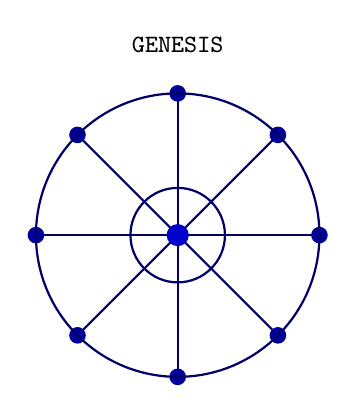
\begin{tikzpicture}
  \foreach \i in {0,...,7} {
    \draw[blue!40!black, thick] (0,0) -- ({45*\i}:1.8);
    \fill[blue!60!black] ({45*\i}:1.8) circle (3pt);
  }
  \draw[blue!40!black, thick] (0,0) circle (1.8);
  \draw[blue!40!black, thick] (0,0) circle (0.6);
  \fill[blue!80!black] (0,0) circle (4pt);
  \node[above] at (0,2.2) {\small\texttt{GENESIS}};
\end{tikzpicture}

\vspace{1cm}
{\Huge\bfseries \ISLS{} Genesis Crystal\\[0.3cm]
v1.0.0}\\[1.5cm]
{\Large The \ADAMANT{} Protocol\\
as Crystallized System Constitution}\\[1cm]
{\large A Machine-Checkable Foundational Artifact\\
for Autonomous, Governed, and Traceable Systems}\\[2cm]
{\large Sebastian Klemm}\\[0.5cm]
{\large 17 March 2026}\\[1.5cm]

\begin{abstract}
\noindent
This document specifies the \emph{Genesis Crystal}: a special Semantic
Crystal that encodes the \ADAMANT{} protocol (Open Projection-Phase-Space
Systems Framework) as a machine-checkable system constitution. The
Genesis Crystal is created at system initialization (\texttt{isls init}),
stored as the first entry in the crystal archive, and validated at
every subsequent run. It contains the architectural axioms, mandatory
invariants, conformance class, operator governance rules, gate
semantics, trace discipline, and security doctrine of the system ---
not as documentation, but as verifiable constraints.

If the system's configuration drifts from its constitutional
commitments, the Genesis Crystal validation fails and every report
shows the violation. The constitution is not a PDF that can be
ignored. It is a crystal that is checked.

No new crate is required. The Genesis Crystal is implemented as
extensions to \texttt{isls-types} (constitutional constraint types),
\texttt{isls-harness} (genesis validation), and \texttt{isls-cli}
(genesis creation and reporting).

\medskip\noindent\textbf{Status:} Implementation Specification.\\
\textbf{Parent:} ISLS v1.0.0 + Extensions Phase 1--5.1.\\
\textbf{Encodes:} \ADAMANT{} Consolidated Master Specification.
\end{abstract}
\end{titlepage}

\tableofcontents
\newpage


%%% =====================================================================
\part{Foundations}\label{part:foundations}

\section{What Is the Genesis Crystal}\label{sec:what}

Every \ISLS{} instance begins with an empty archive. The first crystal
committed to the archive is special: it does not encode a pattern
discovered in data or an artifact forged from intent. It encodes the
\emph{rules by which the system operates}.

\begin{definition}[Genesis Crystal]\label{def:genesis}
The Genesis Crystal $C_0$ is a Semantic Crystal whose
\texttt{constraint\_program} field contains the \ADAMANT{} protocol's
mandatory invariants encoded as machine-checkable predicates. Its
\texttt{topology\_signature} describes the system's architectural
structure at initialization. Its \texttt{evidence\_chain} proves that
the system configuration at initialization satisfies all constitutional
requirements.
\end{definition}

\begin{definition}[Constitutional Constraint]\label{def:constraint}
A constitutional constraint is a predicate $\phi: \mathrm{SystemState}
\to \{0, 1\}$ that encodes one \ADAMANT{} requirement. Each constraint
has:
\begin{itemize}[nosep]
  \item \texttt{id}: unique identifier (e.g., \texttt{"ADAMANT-2.0.1"}),
  \item \texttt{axiom}: the \ADAMANT{} axiom or requirement it encodes,
  \item \texttt{predicate}: the machine-checkable condition,
  \item \texttt{severity}: \texttt{mandatory} or \texttt{recommended},
  \item \texttt{evidence}: what must be present in the system state for
        the predicate to be evaluable.
\end{itemize}
\end{definition}

\begin{axiom}[Constitutional Primacy]\label{ax:primacy}
The Genesis Crystal is the root of all trust. Every other crystal in
the archive is valid only if the Genesis Crystal is valid. If the
Genesis Crystal fails validation, the system \textbf{MUST} report
constitutional violation on every subsequent operation.
\end{axiom}

\begin{axiom}[Immutable Constitution]\label{ax:immutable}
The Genesis Crystal, once committed, \textbf{MUST NOT} be modified,
replaced, or deleted. Constitutional evolution is handled by
\emph{Amendment Crystals} (see \cref{sec:amendment}), not by mutation.
\end{axiom}


\section{When It Is Created}\label{sec:when}

The Genesis Crystal is created exactly once, at system initialization:

\begin{lstlisting}
isls init [--store sqlite] [--profile standard]
\end{lstlisting}

The \texttt{init} command:
\begin{enumerate}[nosep]
  \item Creates the data directory (\texttt{\~{}/.isls/}).
  \item Initializes the archive, store, and config.
  \item Reads the current configuration and registry state.
  \item Evaluates all constitutional constraints against the current state.
  \item If all mandatory constraints pass: commits the Genesis Crystal.
  \item If any mandatory constraint fails: aborts initialization with
        a diagnostic listing which constraints failed and why.
\end{enumerate}


%%% =====================================================================
\part{The Constitutional Constraints}\label{part:constraints}

\section{Mapping \ADAMANT{} to Machine Predicates}\label{sec:mapping}

The following table maps each \ADAMANT{} axiom or requirement to a
concrete, machine-checkable predicate on the \ISLS{} system state.

\begin{longtable}{l l p{5.5cm} l}
\toprule
\textbf{ID} & \textbf{\ADAMANT{} Source} & \textbf{Predicate} &
  \textbf{Severity} \\
\midrule
\endfirsthead \midrule \endhead \bottomrule \endfoot

GC-01 & Axiom 2.0.1 & State domain is bounded:
  all embeddings normalized to $[0,1]^5$ or explicit normalization
  declared in config. & mandatory \\

GC-02 & Axiom 2.0.2 & Every operator in the registry declares
  domain, codomain, admissibility predicate, and version. & mandatory \\

GC-03 & Axiom 2.0.3 & Trace schema is active: every macro-step
  produces a TraceEntry with input digest, state digest, gate
  snapshot. & mandatory \\

GC-04 & Axiom 2.0.4 & Extension crates (C12+) do not override
  kernel invariants I1--I20. Verified by: all 20 AT tests
  referenced in the registry. & mandatory \\

GC-05 & Axiom 2.0.5 & Kernel crates (C1--C11) and extension crates
  (C12+) are structurally separated: no circular dependencies
  from extensions back into kernel. & mandatory \\

GC-06 & R-STATE-001 & Config declares: dimensionality (5),
  normalization rule, component partitioning (p, $\rho$, $\omega$,
  $\chi$, $\eta$), initialization rule, persistence semantics. &
  mandatory \\

GC-07 & R-COH-002 & Coherence functional is bounded $\in [0,1]$,
  decomposed into at least two components (structural +
  temporal), and documented in the registry. & mandatory \\

GC-08 & \S3.4.4 Gate & Gate function produces outcomes from
  $\{\text{reject}, \text{hold}, \text{accept}\}$ (or
  $\{\text{reject}, \text{accept}\}$ for minimal conformance).
  Gate depends on coherence and at least one additional criterion.
  Gate is auditable. & mandatory \\

GC-09 & \S3.6 Cycle & The canonical control cycle exists: Perceive
  $\to$ Focus $\to$ Evaluate $\to$ Gate $\to$ Act $\to$ Trace.
  Verified by: macro\_step implements all phases. & mandatory \\

GC-10 & \S5.1 Invariant & All 8 crystal validation checks are
  active: content\_address, dual\_consensus, evidence\_chain,
  free\_energy, gate\_kairos, immutability, operator\_versions,
  por\_trace. & mandatory \\

GC-11 & \S6.3 Trace & Every committed crystal has a complete
  evidence chain. No crystal exists without trace. & mandatory \\

GC-12 & \S6.6 Replay & Run Descriptor contains sufficient
  information for deterministic replay: seed, config, registry
  digests, scheduler config. & mandatory \\

GC-13 & \S7.2 Proof & Obligation registry (C12) contains at least
  the 8 crystal-validation obligations. & mandatory \\

GC-14 & \S11.1 Security & Capsule protocol (C14) is available.
  Secrets are never stored in plaintext in the archive. &
  mandatory \\

GC-15 & \S11.3 Capability & Gateway authentication is configurable.
  Default: disabled (single-operator). When enabled: bearer token
  required. & recommended \\

GC-16 & \S12.2 Budget & Compute budgets are declared for topology
  (C16), scale (C18), and PMHD (C21). Budget exhaustion triggers
  graceful fallback, not crash. & mandatory \\

GC-17 & \S13.2 Cross-Layer & No emission bypasses the gate. Verified
  by: every code path that produces a crystal goes through the
  gate cascade. & mandatory \\

GC-18 & \S14.1 Policy & Master policy exists: operator execution
  order is deterministic, tie-breaks are declared in RD, no hidden
  state. & mandatory \\

GC-19 & \S16.1 Adaptation & Self-modification (morphogenic
  controller C8) is bounded: max merges per tick, max parameter
  drift per epoch. & mandatory \\

GC-20 & \S20 Epistemic & ``Coherence is not truth'' principle:
  the system does not claim its crystals represent external truth.
  Crystals represent structural invariance relative to observed
  data. & mandatory \\

GC-21 & \S18 Oversight & Human operator can stop the engine at any
  time (Ctrl+C, POST /engine/stop). No autonomous action is
  irreversible without operator confirmation (shadow mode). &
  mandatory \\

\end{longtable}


\section{Conformance Classes}\label{sec:conformance}

Following \ADAMANT{} \S5.2, the Genesis Crystal declares a
conformance class:

\begin{definition}[Conformance Classes]\label{def:confclass}
\begin{itemize}[nosep]
  \item \textbf{C0 --- Minimal}: GC-01 through GC-03 satisfied.
        System can observe and trace.
  \item \textbf{C1 --- Governed}: C0 + GC-04 through GC-09.
        System has operator governance, gate, and cycle.
  \item \textbf{C2 --- Auditable}: C1 + GC-10 through GC-13.
        Full crystal validation, replay, proof obligations.
  \item \textbf{C3 --- Secured}: C2 + GC-14 through GC-16.
        Capsule protocol, authentication, budgets.
  \item \textbf{C4 --- Constitutional}: C3 + GC-17 through GC-21.
        Full \ADAMANT{} compliance including epistemic integrity
        and human oversight.
\end{itemize}
The Genesis Crystal records which class the system satisfies at
initialization.
\end{definition}


%%% =====================================================================
\part{Crystal Structure}\label{part:structure}

\section{Genesis Crystal Schema}\label{sec:schema}

\begin{lstlisting}[title={Genesis Crystal Structure}]
pub struct GenesisCrystal {
    // Standard SemanticCrystal fields
    pub crystal_id: Hash256,
    pub stability_score: f64,        // 1.0 (constitutional)
    pub free_energy: f64,            // -(constraint_count) * 1.0
    pub constraint_program: Vec<ConstitutionalConstraint>,
    pub topology_signature: SystemTopology,
    pub evidence_chain: Vec<EvidenceEntry>,
    pub operator_versions: BTreeMap<String, String>,
    pub created_at_tick: u64,        // 0 (genesis)
    pub carrier_instance: u64,       // 0

    // Genesis-specific fields
    pub adamant_version: String,     // "1.0.0"
    pub conformance_class: ConformanceClass,
    pub system_fingerprint: SystemFingerprint,
    pub constitutional_digest: Hash256,
}

pub struct ConstitutionalConstraint {
    pub id: String,                  // "GC-01" through "GC-21"
    pub axiom_ref: String,           // ADAMANT reference
    pub description: String,         // human-readable
    pub severity: ConstraintSeverity,
    pub satisfied: bool,             // at genesis time
    pub evidence: String,            // JSON proof
}

pub enum ConformanceClass { C0, C1, C2, C3, C4 }

pub enum ConstraintSeverity { Mandatory, Recommended }

pub struct SystemFingerprint {
    pub isls_version: String,
    pub crate_count: usize,
    pub test_count: usize,
    pub registry_digest: Hash256,
    pub config_digest: Hash256,
    pub platform: String,
    pub rust_version: String,
    pub git_commit: Option<String>,
}

pub struct SystemTopology {
    pub crate_graph: BTreeMap<String, Vec<String>>,  // crate -> dependencies
    pub kernel_crates: Vec<String>,                  // C1-C11
    pub extension_crates: Vec<String>,               // C12+
    pub circular_dependencies: Vec<(String, String)>, // must be empty
}
\end{lstlisting}


\section{Genesis Crystal Construction}\label{sec:construction}

\begin{algorithm}[H]
\caption{\textsc{BuildGenesisCrystal}: Construct the system constitution}
\label{alg:genesis}
\begin{algorithmic}[1]
\REQUIRE Config $\theta$, RegistrySet $\calR$, system metadata
\ENSURE GenesisCrystal $C_0$ or initialization failure
\STATE $\mathrm{constraints} \gets \textsc{LoadConstitutionalConstraints}()$
\STATE $\mathrm{fingerprint} \gets \textsc{ComputeSystemFingerprint}(\theta, \calR)$
\STATE $\mathrm{topology} \gets \textsc{ComputeSystemTopology}()$
\STATE \textit{// Evaluate all constraints}
\FOR{each $\phi \in \mathrm{constraints}$}
  \STATE $\phi.\mathrm{satisfied} \gets \textsc{EvaluateConstraint}(\phi, \theta, \calR, \mathrm{topology})$
  \STATE $\phi.\mathrm{evidence} \gets \textsc{GatherEvidence}(\phi, \theta, \calR)$
\ENDFOR
\STATE \textit{// Check mandatory constraints}
\STATE $\mathrm{failures} \gets \{\phi : \phi.\mathrm{severity} = \mathrm{Mandatory} \wedge \neg\phi.\mathrm{satisfied}\}$
\IF{$\mathrm{failures} \neq \emptyset$}
  \STATE \textsc{ReportConstitutionalFailure}($\mathrm{failures}$)
  \RETURN $\bot$ \COMMENT{initialization aborted}
\ENDIF
\STATE \textit{// Determine conformance class}
\STATE $\mathrm{class} \gets \textsc{DetermineConformanceClass}(\mathrm{constraints})$
\STATE \textit{// Build the crystal}
\STATE $C_0 \gets \textsc{BuildCrystal}(\mathrm{constraints}, \mathrm{fingerprint},
  \mathrm{topology}, \mathrm{class})$
\STATE \textit{// Validate through standard 8-gate cascade}
\STATE $\textsc{Validate8Gate}(C_0)$ \COMMENT{must pass}
\STATE \textit{// Commit as first archive entry}
\STATE $\textsc{ArchiveCommit}(C_0)$
\RETURN $C_0$
\end{algorithmic}
\end{algorithm}

\begin{requirement}[Genesis is First]\label{req:first}
The Genesis Crystal \textbf{MUST} be the first entry in the archive.
Its \texttt{created\_at\_tick} is 0. Its commit index is 0. No other
crystal may have commit index 0.
\end{requirement}

\begin{requirement}[Genesis Passes 8 Gates]\label{req:8gate}
The Genesis Crystal itself \textbf{MUST} pass all 8 formal validation
checks. It is a valid Semantic Crystal in every respect. The
constitutional constraints are encoded in its
\texttt{constraint\_program}. Its \texttt{free\_energy} is negative
(computed as $-|\mathrm{constraints}| \cdot 1.0$). Its evidence chain
is complete.
\end{requirement}


%%% =====================================================================
\part{Runtime Validation}\label{part:validation}

\section{Genesis Validation}\label{sec:genesisval}

At every \texttt{validate formal} run, the validation harness includes
a special Genesis check:

\begin{definition}[Genesis Validation]\label{def:genesisval}
Genesis validation consists of three checks:
\begin{enumerate}[nosep,label=(GV\arabic*)]
  \item \textbf{Existence}: the archive contains a crystal with
        \texttt{created\_at\_tick = 0}. If absent, the system was
        not properly initialized.
  \item \textbf{Integrity}: the Genesis Crystal passes the standard
        8-gate validation (content address, evidence chain, etc.).
  \item \textbf{Conformance}: re-evaluate all 21 constitutional
        constraints against the \emph{current} system state. If any
        mandatory constraint that was satisfied at genesis is now
        violated, report constitutional drift.
\end{enumerate}
\end{definition}

\begin{definition}[Constitutional Drift]\label{def:drift}
Constitutional drift occurs when the system's current configuration
no longer satisfies a mandatory constraint that the Genesis Crystal
claims was satisfied at initialization. Causes include:
\begin{itemize}[nosep]
  \item Operator added to the engine but not registered in the
        registry (GC-02 violation).
  \item Gate disabled or threshold set to 0 (GC-08/GC-10 violation).
  \item Trace schema disabled (GC-03 violation).
  \item Compute budget removed (GC-16 violation).
  \item Shadow mode disabled without operator acknowledgment
        (GC-21 violation).
\end{itemize}
\end{definition}

\begin{requirement}[Drift Reporting]\label{req:driftreport}
When constitutional drift is detected, the system \textbf{MUST}:
\begin{enumerate}[nosep,label=(\alph*)]
  \item add a \texttt{CONSTITUTIONAL\_DRIFT} alert to the alert log
        with severity \texttt{red},
  \item include the drift details in every subsequent HTML report
        as a prominent warning banner,
  \item continue operating (the system does not self-halt), but
  \item mark every crystal produced after drift detection with
        \texttt{conformance\_status: "drifted"} in its metadata.
\end{enumerate}
The system does not enforce conformance. It makes non-conformance
visible and indelible.
\end{requirement}


\section{Genesis in Reports}\label{sec:reports}

\begin{definition}[Report Genesis Section]\label{def:reportsection}
The HTML report (\texttt{report full-html}) includes a dedicated
Genesis section:

\begin{lstlisting}[title={Genesis Section in HTML Report}]
Section 0: System Constitution
  Genesis Crystal ID: <truncated hash>
  ADAMANT Version: 1.0.0
  Conformance Class: C4 (Constitutional)
  Created: 2026-03-17T04:20:00Z
  
  Constitutional Constraints: 21/21 satisfied
  
  | ID    | Axiom       | Status | Evidence         |
  |-------|-------------|--------|------------------|
  | GC-01 | Axiom 2.0.1 | PASS   | R5 normalized    |
  | GC-02 | Axiom 2.0.2 | PASS   | 47 ops registered|
  | ...   | ...         | ...    | ...              |
  | GC-21 | S18         | PASS   | shadow mode on   |
  
  Constitutional Drift: NONE
  
  System Fingerprint:
    ISLS v1.0.0 | 24 crates | 243 tests
    Registry: <digest> | Config: <digest>
    Platform: windows | Rust: 1.90.0
    Git: <commit>
\end{lstlisting}

If drift is detected:
\begin{lstlisting}
  Constitutional Drift: DETECTED
  
  | GC-02 | Axiom 2.0.2 | DRIFT | operator "custom_op"
  |       |             |       | not in registry     |
\end{lstlisting}
\end{definition}


%%% =====================================================================
\part{Constitutional Amendment}\label{part:amendment}

\section{Amendment Crystals}\label{sec:amendment}

The Genesis Crystal is immutable. But systems evolve. When the
constitutional commitments need to change (e.g., a new invariant is
added, a conformance class is upgraded, or a constraint is relaxed
with justification), the mechanism is an \emph{Amendment Crystal}.

\begin{definition}[Amendment Crystal]\label{def:amendment}
An Amendment Crystal $C_A$ is a Semantic Crystal with:
\begin{itemize}[nosep]
  \item \texttt{constraint\_program}: the amended constraint set
        (full replacement, not delta),
  \item \texttt{sub\_crystal\_ids}: $[C_0.\mathrm{id}]$ (references
        the Genesis Crystal),
  \item \texttt{amendment\_justification}: canonical JSON explaining
        why each changed constraint was changed,
  \item \texttt{new\_conformance\_class}: the conformance class after
        amendment.
\end{itemize}
An Amendment Crystal passes the standard 8-gate validation and is
committed to the archive like any other crystal. The validation
harness uses the \emph{latest amendment} (or the Genesis Crystal if
no amendments exist) as the active constitution.
\end{definition}

\begin{requirement}[Amendment Chain]\label{req:amendchain}
Amendment Crystals form a chain: each references its predecessor
(Genesis or prior amendment) via \texttt{sub\_crystal\_ids}. The
chain is append-only. The complete constitutional history is
always reconstructible from the archive.
\end{requirement}

\begin{requirement}[No Silent Weakening]\label{req:noweaken}
If an Amendment Crystal relaxes a mandatory constraint (changes it
from mandatory to recommended, or removes it), the
\texttt{amendment\_justification} for that constraint \textbf{MUST}
be non-empty. An amendment that silently weakens a constraint without
justification \textbf{MUST} fail validation.
\end{requirement}


%%% =====================================================================
\part{Implementation}\label{part:impl}

\section{Changes to Existing Crates}\label{sec:changes}

\subsection{\texttt{isls-types} Extensions}

\begin{lstlisting}
// New types in isls-types/src/lib.rs

pub struct ConstitutionalConstraint {
    pub id: String,
    pub axiom_ref: String,
    pub description: String,
    pub severity: ConstraintSeverity,
    pub satisfied: bool,
    pub evidence: String,
}

pub enum ConstraintSeverity { Mandatory, Recommended }
pub enum ConformanceClass { C0, C1, C2, C3, C4 }

pub struct SystemFingerprint {
    pub isls_version: String,
    pub crate_count: usize,
    pub test_count: usize,
    pub registry_digest: Hash256,
    pub config_digest: Hash256,
    pub platform: String,
    pub rust_version: String,
    pub git_commit: Option<String>,
}

pub struct GenesisMetadata {
    pub adamant_version: String,
    pub conformance_class: ConformanceClass,
    pub system_fingerprint: SystemFingerprint,
    pub constitutional_digest: Hash256,
    pub constraints: Vec<ConstitutionalConstraint>,
}
\end{lstlisting}

\subsection{\texttt{isls-harness} Extensions}

\begin{lstlisting}
// New module: isls-harness/src/genesis.rs

pub fn build_genesis_crystal(
    config: &Config,
    registries: &RegistrySet,
) -> Result<SemanticCrystal, GenesisError>;

pub fn evaluate_constitutional_constraints(
    config: &Config,
    registries: &RegistrySet,
) -> Vec<ConstitutionalConstraint>;

pub fn validate_genesis(
    archive: &Archive,
    config: &Config,
    registries: &RegistrySet,
) -> GenesisValidationResult;

pub struct GenesisValidationResult {
    pub exists: bool,
    pub integrity: bool,          // 8-gate check
    pub conformance: bool,        // all mandatory still satisfied
    pub drift: Vec<String>,       // constraint IDs that drifted
    pub conformance_class: ConformanceClass,
}

pub fn detect_constitutional_drift(
    genesis: &SemanticCrystal,
    current_config: &Config,
    current_registries: &RegistrySet,
) -> Vec<DriftEntry>;

pub struct DriftEntry {
    pub constraint_id: String,
    pub was: bool,                // satisfied at genesis
    pub now: bool,                // satisfied now
    pub detail: String,
}
\end{lstlisting}

\subsection{\texttt{isls-cli} Extensions}

\begin{lstlisting}
// Enhanced init command
isls init [--store sqlite] [--profile standard]
// Now creates Genesis Crystal as first archive entry

// New genesis commands
isls genesis show          // Display Genesis Crystal summary
isls genesis validate      // Run GV1-GV3 checks
isls genesis amend --justification amend.json
                           // Create an Amendment Crystal

// Enhanced validate command
isls validate formal       // Now includes Genesis validation
isls validate genesis      // Genesis-specific validation

// Enhanced report
isls report full-html      // Now includes Section 0: Constitution
\end{lstlisting}

\subsection{\texttt{isls-store} Extension}

\begin{lstlisting}
// New table for constitutional history

CREATE TABLE constitution (
    crystal_id    TEXT PRIMARY KEY,
    is_genesis    BOOLEAN NOT NULL,
    is_amendment  BOOLEAN NOT NULL,
    conformance   TEXT NOT NULL,     -- 'C0'..'C4'
    constraints   TEXT NOT NULL,     -- JSON array
    created_at    TEXT NOT NULL
);

// Query: get active constitution
// (latest amendment, or genesis if no amendments)
pub fn get_active_constitution(&self) -> Result<ConstitutionRow>;
\end{lstlisting}


%%% =====================================================================
\part{Acceptance Tests}\label{part:tests}

\begin{longtable}{l l p{6.5cm}}
\toprule
\textbf{ID} & \textbf{Name} & \textbf{Procedure} \\
\midrule
\endfirsthead \midrule \endhead \bottomrule \endfoot
AT-G1 & Genesis creation & Run \texttt{isls init}; verify archive
  contains exactly one crystal with tick=0. \\
AT-G2 & Genesis 8-gate & Validate the Genesis Crystal; verify all
  8 checks pass. \\
AT-G3 & Genesis constraints & Inspect Genesis Crystal; verify 21
  constraints present, all mandatory ones satisfied. \\
AT-G4 & Conformance class & With default config, verify conformance
  class is C4. \\
AT-G5 & Constitutional drift & After genesis, modify config to
  disable trace; run \texttt{validate genesis}; verify GC-03 drift
  detected. Restore config; verify drift clears. \\
AT-G6 & Missing genesis & Delete genesis crystal from archive; run
  \texttt{validate formal}; verify GV1 failure reported. \\
AT-G7 & Amendment crystal & Create amendment that adds a constraint;
  verify amendment references genesis; verify new constraint
  checked on subsequent validation. \\
AT-G8 & No silent weakening & Create amendment that removes a
  mandatory constraint without justification; verify amendment
  fails validation. \\
AT-G9 & Genesis in report & Generate HTML report; verify Section~0
  present with constraint table and fingerprint. \\
AT-G10 & Double init prevention & Run \texttt{isls init} on an
  already-initialized system; verify error ``genesis already
  exists.'' \\
\end{longtable}


%%% =====================================================================
\part{Handoff}\label{part:handoff}

\section{Test Count}

\begin{tabular}{l r r}
\toprule
\textbf{Phase} & \textbf{New Tests} & \textbf{Cumulative} \\
\midrule
Phase 1--5.1 & 231 & 231 \\
Genesis Crystal & 10 & $\ge$ 241 \\
\bottomrule
\end{tabular}

\section{Verification Sequence}

\begin{lstlisting}
# Build
cargo build --workspace --release 2>&1 | grep -c warning  -> 0

# Test
cargo test --workspace -- --test-threads=1  -> >= 241 passed

# Initialize with Genesis Crystal
rm -rf ~/.isls
cargo run --bin isls --release -- init

# Verify Genesis exists and is valid
cargo run --bin isls --release -- genesis show
cargo run --bin isls --release -- genesis validate
# -> Genesis Crystal: VALID, Conformance: C4, 21/21 constraints

# Run a scenario
cargo run --bin isls --release -- ingest --adapter synthetic --scenario S-Basic
cargo run --bin isls --release -- run --mode shadow --ticks 100

# Validate includes Genesis check
cargo run --bin isls --release -- validate formal
# -> Genesis: VALID | Crystals: 50/50 pass

# Generate report with Section 0
cargo run --bin isls --release -- report full-html
# -> Section 0: System Constitution present

# Test drift detection
# (temporarily modify a config value that violates GC-XX)
cargo run --bin isls --release -- genesis validate
# -> DRIFT DETECTED: GC-XX
\end{lstlisting}

\section{Completion Criteria}

The Genesis Crystal specification is complete when:
\begin{enumerate}[nosep]
  \item \texttt{isls init} creates a Genesis Crystal as the first
        archive entry.
  \item The Genesis Crystal passes all 8 formal validation checks.
  \item All 21 constitutional constraints are evaluated and encoded.
  \item Conformance class is correctly determined.
  \item Constitutional drift is detected when config changes.
  \item Amendment Crystals work and reference the Genesis.
  \item HTML report includes Section~0: System Constitution.
  \item All 10 acceptance tests pass.
  \item Total tests $\ge 241$, zero warnings.
\end{enumerate}


\vfill
\begin{center}
\rule{0.5\textwidth}{0.4pt}\\[0.5cm]

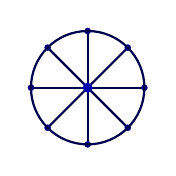
\begin{tikzpicture}[scale=0.6]
  \foreach \i in {0,...,7} {
    \draw[blue!30!black, thick] (0,0) -- ({45*\i}:1.2);
    \fill[blue!50!black] ({45*\i}:1.2) circle (2pt);
  }
  \draw[blue!30!black, thick] (0,0) circle (1.2);
  \fill[blue!70!black] (0,0) circle (3pt);
\end{tikzpicture}

\vspace{0.3cm}
{\small Generated for \ISLS{} Genesis Crystal v1.0.0.\\
The constitution is not a document. It is a crystal.\\
It is not read. It is checked.\\[0.3cm]
Deterministic, append-only, replay-verified.\\
\ADAMANT{}.}
\end{center}

\end{document}
